\section{Nyquist-Shannon Theorem}
\label{sec:nyquistshannon}

 Wie in \cite[Kap. 2]{lyons2011} beschrieben, gibt es für jede Folge an abgetasteten Werten unendlich viele
 Möglichkeiten, dieses Signal zu interpretieren. Die ursprüngliche Frequenz des Signals wird periodisch und unendlich oft ober- und unterhalb
 der jeweiligen Frequenz gespiegelt (auch \textit{Aliasing} genannt) \cite[Kapitel 2]{lyons2011},
 veranschaulicht in Abbildung \ref{fig:aliasing}.


 Mathematisch genau lässt sich dieses Phänomen wie folgt beschreiben:
 \begin{equation}
    x[n] = \sin(2\pi \cdot f_0 \cdot n \cdot t_s) = \sin(2\pi \cdot (f_0 + k \cdot f_s) \cdot n \cdot t_s)
    \label{eq:Aliasing}
 \end{equation}
 wobei:
 \begin{itemize}
    \item[$f_0$]: Ursprungsfrequenz in Hz
    \item[$f_s$]: Abtastfrequenz in Hz 
    \item[$n \in \mathbb{N}$]: Index der Folge von abgetasteten Werten
    \item[$k \in \mathbb{Z}$]: Faktor, der die unendlichen spektralen Wiederholungen beschreibt
 \end{itemize}
 Die Faktoren $f_0$ und $(f_0 + kf_s)$ führen also zum gleichen Ergebnis an Signalwerten.

 Der mathematische Beweis dafür wird hier übersprungen, da es den Rahmen sprengen würde\cite[vgl. Kap 2]{lyons2011}
 Um mit dieser Problematik umzugehen, bedient man sich der sog. \textit{Nyquist-Frequenz} oder auch \textit{Nyquist-Grenze}
 , die wie folgt definiert ist:
 \begin{equation}
    f_{Nyquist} = \frac{f_s}{2}
    \label{eq:nyquist_border}
 \end{equation}
 wobei $f_s$ wieder für die Abtastfrequenz steht.

 \begin{figure}[!htpb]
    \centering
    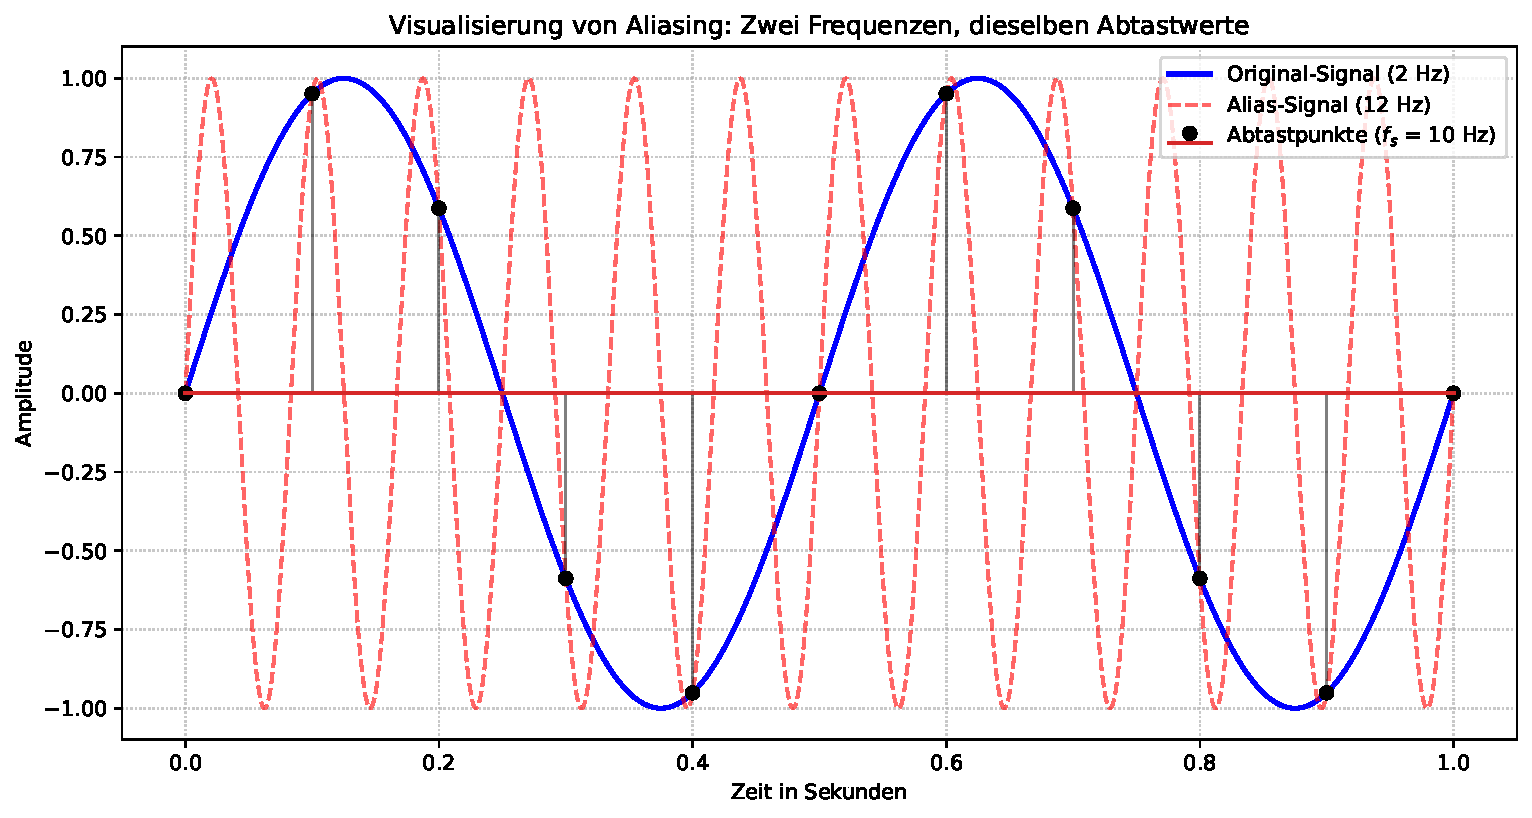
\includegraphics[width = 0.5\textwidth, height=4cm]{graphic/python/chapter2/aliasing_vergleich.pdf}
    \caption{Neben den beiden abgebildeten Kurven könnten unendlich viele weitere Kurven über die Abtastwerte gelegt werden}
    \label{fig:aliasing}
 \end{figure}